\documentclass[12pt]{article}
\usepackage[utf8]{inputenc}
\usepackage{polski}
\usepackage{graphicx}
\usepackage{amsmath}
\usepackage{bm}
\usepackage[table]{xcolor}
\usepackage[margin=2.5cm]{geometry}
\usepackage{anyfontsize}
\graphicspath{ {img/} }

\begin{document}
	\begin{titlepage}
		\begin{flushright}
			\Huge DOKUMENTACJA TECHNICZNA
		\end{flushright}
		\hrulefill
		\vspace*{4cm}
		\centering
		
		LABORATORIUM INTERFEJSÓW OBIEKTOWYCH
		\vspace*{0.5cm}
		
		{\fontsize{64}{1.2}\selectfont \textbf{Amperomierz}}
		
		\vspace*{4cm}
		\underline{\normalsize AUTORZY:} \\
		\Large Tomasz \textbf{Masłoń} \\
		\Large Kamil \textbf{Nawrot}
		
		\vspace*{0.5cm}
		
		\underline{\normalsize OPIEKUN:} \\
		\Large mgr inż. Paweł \textbf{Dobrowolski}
		
		\vspace*{\fill}
		
\includegraphics[scale=0.3]{logo.png} \\
		{\footnotesize Wrocław, 2019}
	\end{titlepage}

\newpage

\tableofcontents
\listoffigures
\listoftables

\newpage

\section{Ogólny opis układu}
Realizowany układ elektroniczny miał za zadanie działać jako miernik natężenia prądu stałego z zakresu \textbf{0.1 - 2A}, przetwarzając podawany mu prąd na dwa standardy najczęściej stosowane w przemyśle:
\begin{itemize}
	\item sygnał napięciowy \textbf{0\,\dots10V}
	\item sygnał prądowy \textbf{4\,\dots20mA}
\end{itemize}
Oprócz tego, z wykorzystaniem przetwornika analogowo-cyfrowego \textbf{ICL7107}, zaimplementowano możliwość wyświetlania mierzonej wartości na trzech wyświetlaczach siedmiosegmentowych. Układ oparty został przede wszystkim na wzmacniaczach operacyjnych, które, skalując i przesuwając, przetwarzały sygnał wejściowy do odpowiednich wartości. \\

\section{Założenia projektowe}
\subsection{Zasilanie}
Układ należało zasilić symetrycznym napięciem $\pm$\textbf{12V}, ponieważ zastosowane wzmacniacze operacyjne również wymagają tego typu zasilenia. Konieczne było wyprowadzenie z generatorów trzech sygnałów: napięcia dodatniego, ujemnego oraz odniesienia (0V). 
\subsection{Przetwarzanie wartości mierzonej}
Sygnał mierzony musi być podawany na rezystor pomiarowy $\mathbf{0.1\Omega}$, aby uzyskać znany spadek napięcia, na którym mogą pracować kolejne elementy układu. Konieczna jest odpowiednia polaryzacja. Napięcie z rezystora podawane jest na kolejne wzmacniacze operacyjne, które działają w konfiguracji wzmacniacza nieodwracającego (przeskalowywanie sygnału) lub sumującego albo odejmującego (przesuwanie sygnału o stałą wartość). 
\subsection{Dokładność}
W całym urządzeniu stosowano rezystory z szeregu E24, które charakteryzują się tolerancją rzędu $\pm$5\%. Ich wartości bezpośrednio wpływają na parametr wzmocnienia każdego wzmacniacza oraz mnożniki dzielników napięciowych, w związku z czym w układzie mogą pojawiać się zauważalne różnice pomiędzy wartościami rzeczywistymi a przetworzonymi. W celu redukcji tych błędów, w koniecznych miejscach zastosowano precyzyjne potencjometry, które pozwalają na doregulowanie wartości napięcia. Przy takim rozwiązaniu powinno być możliwe uzyskanie dokładności pomiarów na poziomie 2\%. \\

\section{Koncepcja działania}\label{sec:koncepcja}
\subsection{Sygnał napięciowy 0\,\dots\,10V}\label{subsec:0-10V}
Mierzony prąd podawany jest na opornik pomiarowy. Spadek napięcia na nim może wynosić od 0.01V do 0.2V. Napięcie to kierowane jest na wzmacniacz różnicowy o pięćdziesięciokrotnym wzmocnieniu, zatem na jego wyjściu uzyskuje się napięcie \textbf{0.5-10V}. Kolejnym krokiem jest przesunięcie napięcia w dół o 0.5V z jednoczesnym wzmocnieniem, tak aby uzyskać zakres \textbf{0-10V}. Wzmacniacz realizujący tę operację pracuje w konfiguracji wzmacniacza odejmującego. Stałe napięcie 0.5V pobierane jest ze stabilizowanego zasilania sterownika \textbf{ICL7107} (opisanego w dalszej cześci dokumentacji). Wzmocnienie wynosi około $1.06$, tak aby podnieść górną granicę zakresu z 9.5 na 10V. Tak przetworzony sygnał wyprowadzony jest na złącze, które umożliwia jego pomiar.
\subsection{Sygnał prądowy 4\,\dots\,20mA}\label{subsec:4-20mA}
Napięcie uzyskane na poprzednim wzmacniaczu (0-10V) jest wykorzystywane w celu dalszego przetworzenia. Najpierw, za pomocą dzielnika napięciowego obniża się jego wartość do zakresu \textbf{0-4V}. Analogicznie jak 0.5V uzyskuje się napięcie 1V, które następnie jest dodawane za pomocą wzmacniacza sumującego o wzmocnieniu $1$ do sygnału z poprzedniego wzmacniacza operacyjnego. W ten sposób uzyskuje się wyjściowe napięcie o zakresie \textbf{1-5V}.
\subsection{Wyświetlacze siedmiosegmentowe}\label{subsec:7segmentowe}
Sygnał uzyskany za pierwszym wzmacniaczem operacyjnym układu (omówionym w punkcie \ref{subsec:0-10V}) jest kierowany na kolejny wzmacniacz o odwrotnym wzmocnieniu, który sprowadza sygnał ponownie do zakresu \textbf{0.01 - 0.2V}. Takie napięcie kierowane jest na sterownik wyświetlacza ($V_{in}$). Wymaga on także napięcia odniesienia $V_{ref}$ o wartości 1V, które także zostało uzyskane już wcześniej (punkt \ref{subsec:4-20mA}). ICL7107 wyświetla wartość napięcia uzyskaną ze wzoru:
\begin{equation*}
V_{disp} = 1000 \cdot \frac{V_{in}}{V_{ref}},
\end{equation*}
czyli wartości z zakresu \textbf{010 - 200}.
Koncepcję działania układu przedstawia także schemat blokowy, Załącznik do dokumentacji.

\section{Realizacja zasilania i jego zabezpieczenia}
\subsection{Główne zasilanie układu}
Cały układ zasilany jest stałym napięciem symetrycznym $\pm$12V. Układ połączenia zasilaczy (\textit{rys}) generuje potencjał odniesienia oraz dwie linie o potencjałach +12V i -12V względem masy. Na układ wyprowadzone są więc trzy osobne linie. Szeregowo z napięciem dodatnim połączona jest dioda Schottky'ego \textbf{BAT42}, która zabezpiecza układ przed odwrotnym podłączeniem zasilania. Działa ona analogicznie do zwykłej diody prostowniczej, jednak spadek napięcia na samym elemencie jest dużo niższy (około 0.3V).
\begin{figure}[h]
\centering
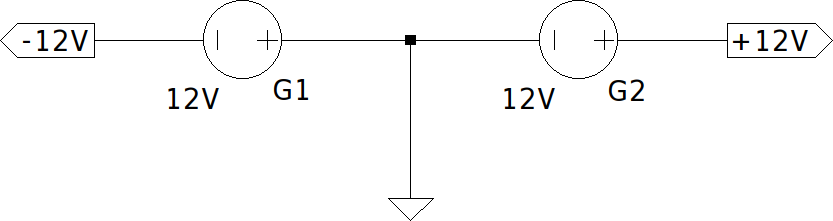
\includegraphics[scale=0.5]{power_supply.png}
\label{main_power_supply}
\caption{Ideowy schemat realizacji głównego zasilania układu}
\end{figure}

\subsection{Zasilanie przetwornika ICL7107}
Sterownik do obsługi wyświetlaczy wymaga zasilania symetrycznego o napięciu 5V. Uzyskuje się je z zasilania głównego z wykorzystaniem diód Zenera o napięciu przebicia równym 5.1V (\textit{rys}). Uzyskiwany w ten sposób spadek napięcia jest stabilny i niezależny od zmian wartości zasilania głównego. Fakt ten wykorzystuje się, używając napięcie zasilające ICL7107 także do uzyskiwania wartości 0.5V i 1V, które potrzebne są przy przesuwaniu zakresów napięcia na wzmacniaczach operacyjnych. Sygnał zasilający jest dodatkowo odfiltrowywany przez kondensatory elektrolityczne 10$\mu$F.
\begin{figure}[h]
\centering
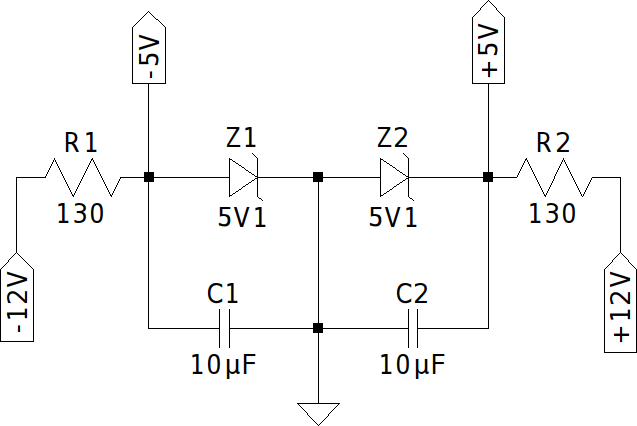
\includegraphics[scale=0.5]{icl_power_supply.png}
\label{icl_power_supply}
\caption{Ideowy schemat realizacji zasilania układu ICL7107}
\end{figure}

\subsection{Zasilanie diód wyświelaczy}
Przyjęto pobór prądu dla każdej czerwonej diody na poziomie 3-4mA. Realizację układu zasilającego przeprowadzono analogicznie jak przy sterowniku (\textit{rys}). Osobne zasilanie zapewnia stabilność zasilania ICL7107 oraz wyjść wtórników napięciowych utrzymujących napięcia 0.5V i 1V, ponieważ pobór prądu przy dużej ilości zapalonych segmentów może być znaczny i mógłby wpływać na inne elementy układu, gdyby zostało wykonane wspólne zasilanie.

\section{Zastosowane elementy i układy elektroniczne}
\subsection{Układy scalone}
\begin{itemize}
	\item wzmacniacz operacyjny \textbf{TL081CP} (\textit{x8}) - przetwarzanie zakresów napięcia, wtórniki napięciowe
	\begin{figure}[h]
	\centering
	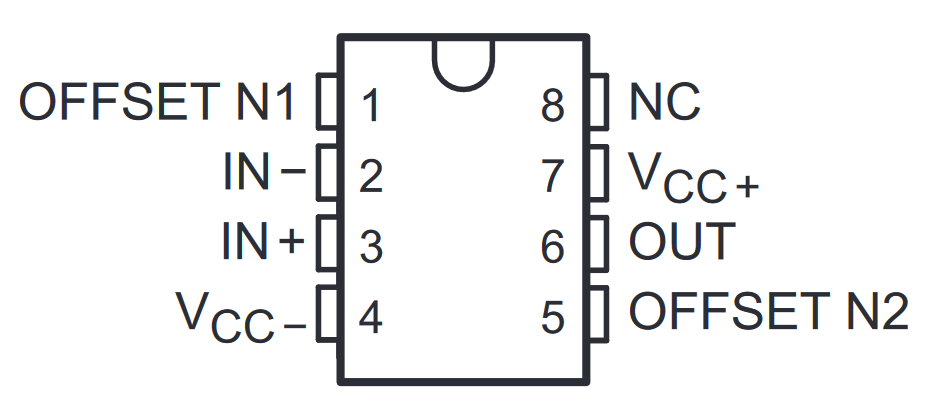
\includegraphics[scale=0.2]{tl081_pinout.png}
	\label{tl081_pinout}
	\caption{Konfiguracja pinów wzmacniacza operacyjnego TL081}
	\end{figure}
	\item przetwornik analogowo-cyfrowy \textbf{ICL7107} - przetwarzanie analogowego sygnału napięciowego na 		cyfrowe sterowanie trzema wyświetlaczami siedmiosegmentowymi
	\begin{figure}[h]
	\centering
	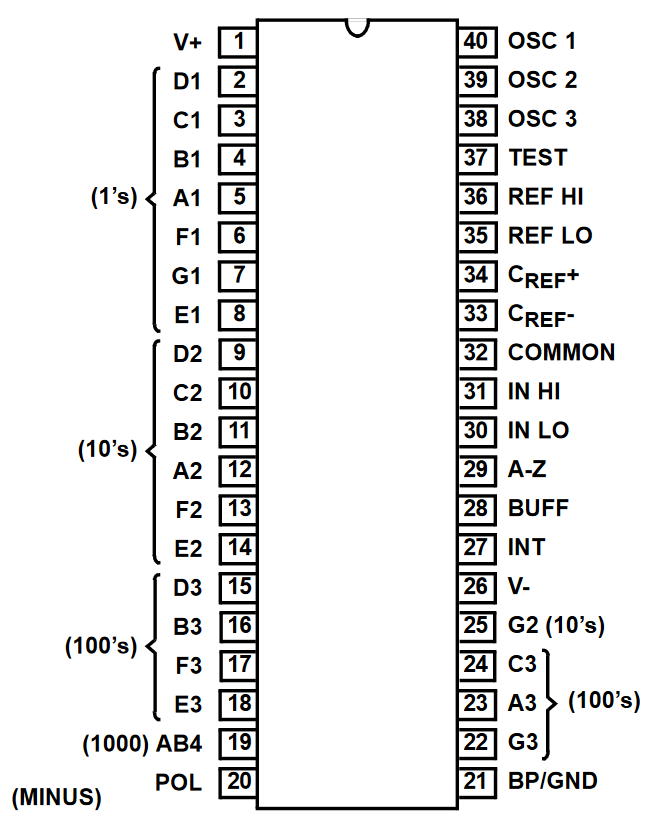
\includegraphics[scale=0.3]{icl7107_pinout.png}
	\label{tl081_pinout}
	\caption{Konfiguracja pinów przetwornika A/C ICL7107}
	\end{figure}
\end{itemize}
\subsection{Elementy półprzewodnikowe}
\begin{itemize}
	\item tranzystor bipolarny typu NPN \textbf{BD139}
	\item dioda Schottky'ego \textbf{BAT42} - zabezpieczenie głównego zasilania przed odwrotną polaryzacją
	\item dioda Zenera 5V1 (\textit{x2}) - stabilizator napięcia zasilającego przetwornik ICL7107
	\item dioda Zenera 5V6 - stabilizator napięcia zasilającego wyświetlacze
\end{itemize}
Wymieniono tylko układy i elementy o większym znaczeniu i bardziej skomplikowanym działaniu. Wykaz wszystkich użytych w projekcie elementów, wraz z podstawowymi parametrami, znajduje się w Załączniku dołączonym do dokumentacji.




\end{document}